Your cell door swings open to the protest of its rusted hinges and the jailer steps inside, drool slavering from his mouth. He raises his torch overhead, filling the cell with its harsh glow. With his other hand, he closes the door behind him--and readjusts his grip on the meat hook. 

\subsection*{Victory Condition}
Defeat the Jailer

\subsection*{Doom Events}
\begin{itemize}
\item \textbf{Round 3:} \emph{Out of the corner of your eye, you notice something--that door didn’t shut all the way.} Hex \emph{5,3} becomes an Escape Tile instead of Impassable Boundary.
\end{itemize}

\subsection*{Encounter Table}
\begin{tcolorbox}
\textbf{Roll:} 1D6
\begin{center}
\begin{tabular}{ L | L | L }
\multicolumn{1}{c|}{\textbf{1}} & 
\multicolumn{1}{c|}{\textbf{2-5}} & 
\multicolumn{1}{c}{\textbf{6}} \\
\emph{Torch Flurry} &
Move. \emph{Meat Hook}\newline \emph{This result is only exhausted after its third token} &
\textbf{A:} \emph{Sudden. Strong Kick}\newline \textbf{B:} Move. \emph{Meat Hook}
\end{tabular}
\end{center}
\end{tcolorbox}

\begin{tcolorbox}
\textbf{Note:} Remember that the \emph{Sudden} tag on behavior 6-A means the character will not be able to commit a reaction. However, if the jailer cannot resolve 6-A then 6-B does not have the \emph{Sudden} tag.
\end{tcolorbox}

\subsection*{Enemy Sheet}
\hrule
\ \\
{\large \textbf{The Jailer}}\\\\
\begin{tabular}{s s}
\textbf{HP:} 7 & \textbf{Move:} 2\\
\end{tabular}\\

\emph{Hollow:} This entity ignores the Stunned, Charmed, Maddened, and Fear conditions.\\

\emph{Hungering Pursuit:} The character may not commit Escape if this entity occupies an adjacent tile.\\

\textbf{Attacks:}
\begin{itemize}
\item \emph{Meat Hook} - Deal 1 Pierce damage to an adjacent entity.
\item \emph{Strong Kick} - Move 1. Deal 1 \emph{Unparryable} Crush damage and Knockback 1 to an adjacent entity.
\item \emph{Torch Flurry} - Deal 1 Burn damage to an adjacent entity. Resolve this attack three times.
\end{itemize}
\hrule

\begin{tcolorbox}
\textbf{Hint:} Remember that \emph{Torch Flurry} is resolved three times, so a \emph{Dodge!} would only negate one of those three attacks. However, the player may commit \emph{Dodge!} before each attack if they have the \textbf{SP} dice to do so (or if their \emph{Dodge!} has implicit Move they could use it to get out of range).
\end{tcolorbox}

\subsection*{Encounter Map}

\begin{center}
\framebox{
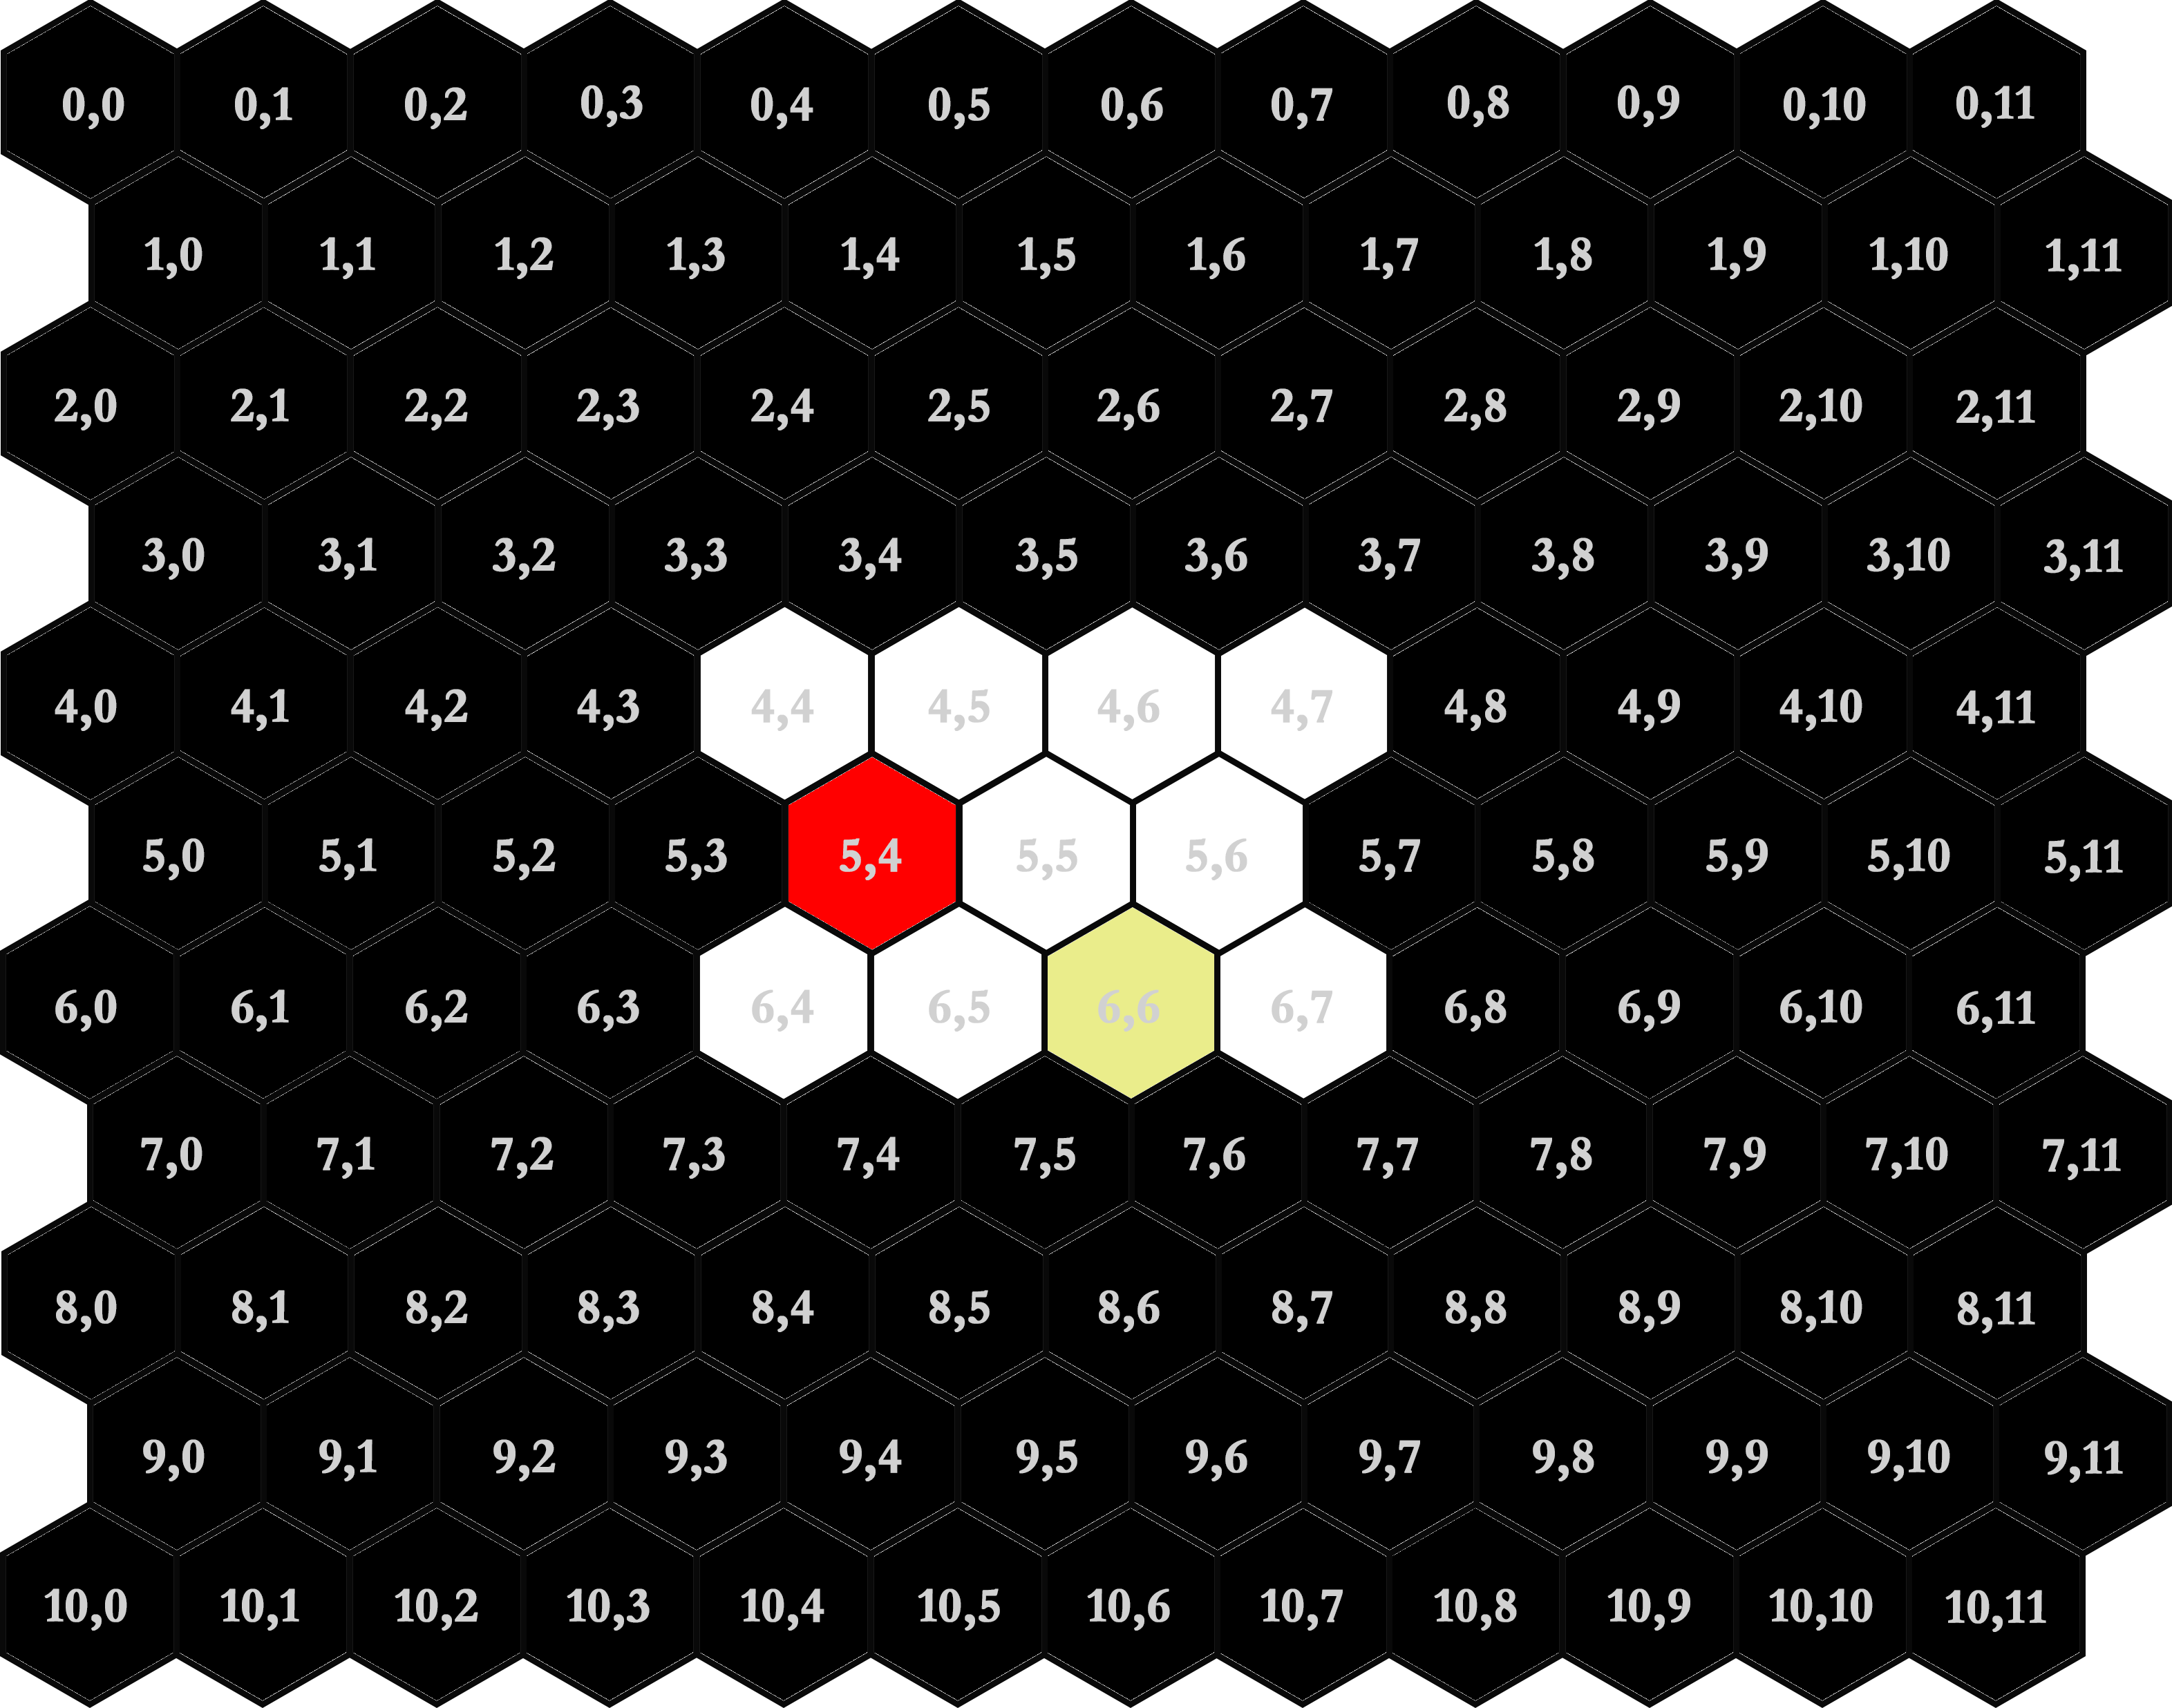
\includegraphics[width = 0.96\textwidth]{./maps/c12.png}
}
\end{center}

\subsection*{Setup Instructions}
\begin{itemize}
\item \textbf{Goldenrod:} Character Start Location.
\item \textbf{Red:} Jailer Start Location.
\item \textbf{Black:} Impassable Boundary.
\item \textbf{Not Pictured:} Escape Tile.
\end{itemize}

\begin{tcolorbox}
\textbf{Hint:} When setting up the Hexagon-Tiled Map for an encounter, it’s best to use light marks so that they can be erased (and the map re-used) later. In this case, it isn’t necessary to fill in each and every impassable boundary tile. Drawing a bounding box around the relevant tiles is sufficient. This will also help to cutdown on setup time.
\end{tcolorbox}

\pagebreak

\begin{tcolorbox}
\textbf{Note:} Whenever the character receives souls (exact value in parentheses) total them onto the character sheet. The soul name is purely for flavor text, only the parenthesized value matters.
\end{tcolorbox}

\subsection*{Victory}
The jailer lets out a bout of manic laughter, and then sets himself alight with his own torch. He flails about the cell for a moment, engulfed in flames, before finally collapsing with one last chuckle. As he expires, you feel a strange sensation wash over you: not mere relief, nor the thrill of vengeance. You are... stronger, somehow.\\
>> Soul of a Madman (8)\\
\gain{Torch}\\
\gain{Meat Hook}\\
\notegain{c12a} Jailer’s Keychain\\
>> \turnto{c13}

\begin{tcolorbox}
\textbf{Note:} When given the option to collect equipment, either equip it immediately or add it to the 8 \emph{carried} slots on the record sheet. Equipment found outside of encounters can be left behind and collected later. There’s no incentive to hoard gear.
\end{tcolorbox}

\subsection*{Defeat}
You lie in defeat, your blood pooling along the mortar lines. The jailer plants a boot on your chest, gasping from all his laughter. Spittle flecks across your face as he raises the meat hook and...\\

And then you startle awake. Your sweat-soaked rags, cooled by the damp cell, send a shiver down your spine. When your eyes adjust to the dim light, you realize something peculiar: your cell door is wide open. Risking a glance outside, you discover that the hall is deserted as well. A stroke of good fortune, or a sign of something dire happening in the prison? Perhaps the two are one in the same.\\

>> Clear all \textbf{HP} slots of damage tokens.\\
\notegain{c12b} Woke up in an unlocked cell\\
>> \turnto{c13}

\subsection*{Retreat}
You slip into the hallway and slam the cell door behind you. The jailer throws himself up against the other side, his instruments clattering to the floor. For a moment, the two of you stare across the slit window. A brief look of clarity shows on his face, as if the hollow realized the grim irony of his situation. But then the light fades from his eyes again, and he shuffles off into a corner, mumbling to himself.\\

Doubtless, he will eventually realize that he holds the keys to his own cell. But the cogs of a maddened mind often wheel in the wrong direction; that might be a long time coming indeed.\\

\notegain{c12c} Trapped the jailer\\
>> \turnto{c13}